\documentclass[ignorenonframetext,]{beamer}
\usetheme{Warsaw}
\usefonttheme{serif}
\setbeamertemplate{caption}[numbered]
\setbeamertemplate{caption label separator}{:}
\setbeamercolor{caption name}{fg=normal text.fg}
\usepackage{amssymb,amsmath}
\usepackage{ifxetex,ifluatex}
\usepackage{fixltx2e} % provides \textsubscript
\usepackage{lmodern}
\ifxetex
  \usepackage{fontspec,xltxtra,xunicode}
  \defaultfontfeatures{Mapping=tex-text,Scale=MatchLowercase}
  \newcommand{\euro}{€}
\else
  \ifluatex
    \usepackage{fontspec}
    \defaultfontfeatures{Mapping=tex-text,Scale=MatchLowercase}
    \newcommand{\euro}{€}
  \else
    \usepackage[T1]{fontenc}
    \usepackage[utf8]{inputenc}
      \fi
\fi
% use upquote if available, for straight quotes in verbatim environments
\IfFileExists{upquote.sty}{\usepackage{upquote}}{}
% use microtype if available
\IfFileExists{microtype.sty}{\usepackage{microtype}}{}
\usepackage{graphicx}
\makeatletter
\def\maxwidth{\ifdim\Gin@nat@width>\linewidth\linewidth\else\Gin@nat@width\fi}
\def\maxheight{\ifdim\Gin@nat@height>\textheight0.8\textheight\else\Gin@nat@height\fi}
\makeatother
% Scale images if necessary, so that they will not overflow the page
% margins by default, and it is still possible to overwrite the defaults
% using explicit options in \includegraphics[width, height, ...]{}
\setkeys{Gin}{width=\maxwidth,height=\maxheight,keepaspectratio}

% Comment these out if you don't want a slide with just the
% part/section/subsection/subsubsection title:
\AtBeginPart{
  \let\insertpartnumber\relax
  \let\partname\relax
  \frame{\partpage}
}
\AtBeginSection{
  \let\insertsectionnumber\relax
  \let\sectionname\relax
  \frame{\sectionpage}
}
\AtBeginSubsection{
  \let\insertsubsectionnumber\relax
  \let\subsectionname\relax
  \frame{\subsectionpage}
}

\setlength{\parindent}{0pt}
\setlength{\parskip}{6pt plus 2pt minus 1pt}
\setlength{\emergencystretch}{3em}  % prevent overfull lines
\setcounter{secnumdepth}{0}

\title{Stevens Institute of Technology Summer Project}
\author{Andrea García Tapia}
\date{07/03/15}

\begin{document}
\frame{\titlepage}

\begin{frame}{Introduction}

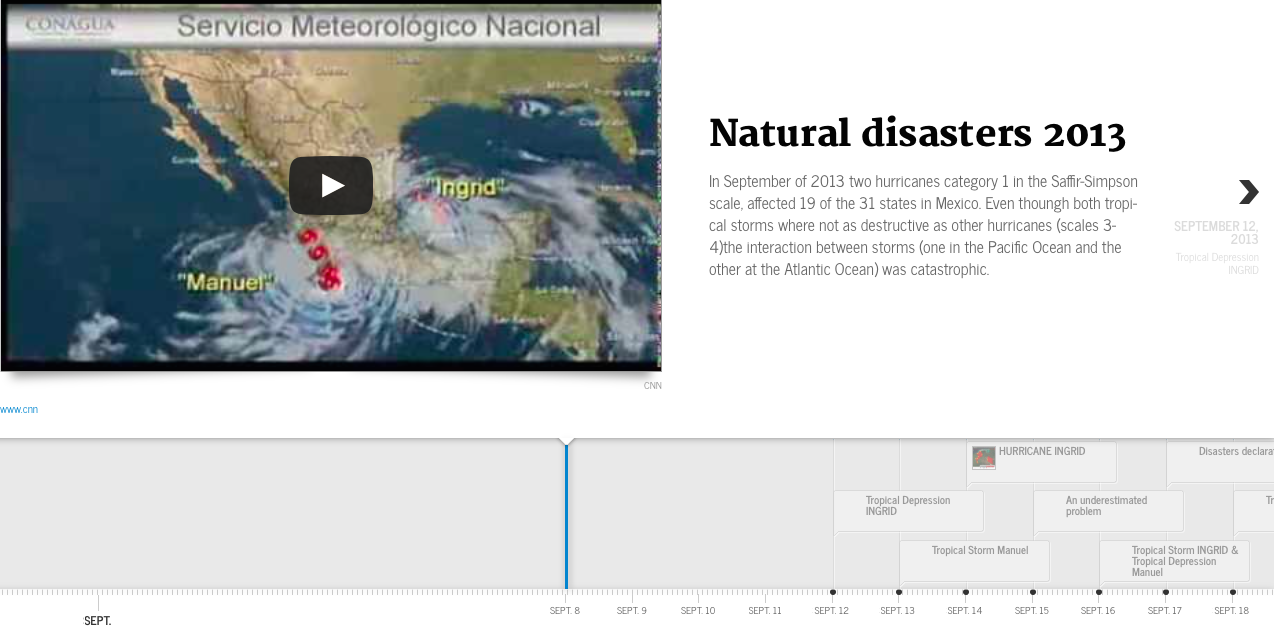
\includegraphics{img/timeline.png}

Follow the
\href{http://cdn.knightlab.com/libs/timeline/latest/embed/index.html?source=1wesPOVIPMQLbCplDyt5ENxd_H74QPUYk1GuBslD1mFY\&font=Merriweather-NewsCycle\&maptype=toner-lines\&lang=en\&height=650}{Disaster
Time Line} to learn more about the evolution of Ingrid and Manuel
tropical storms.

\end{frame}

\begin{frame}{Disaster Risk Management}

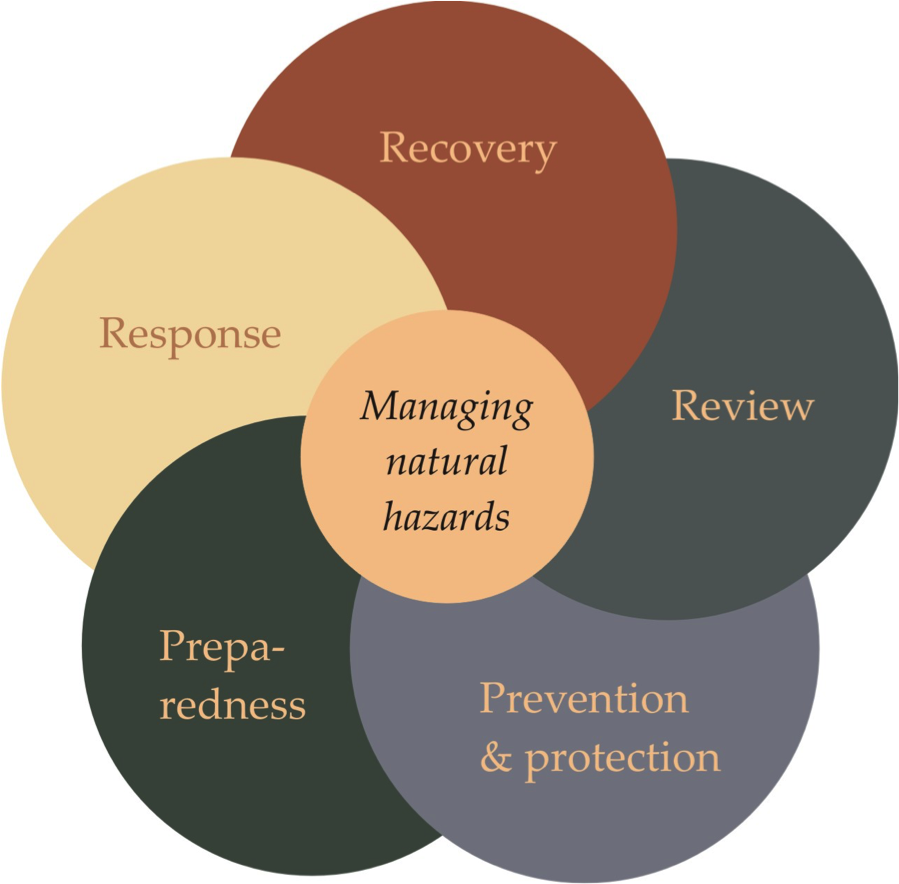
\includegraphics{img/rmc.png}

source: CATALYST winter Resilience Academy, 2013

\end{frame}

\begin{frame}{Problem}

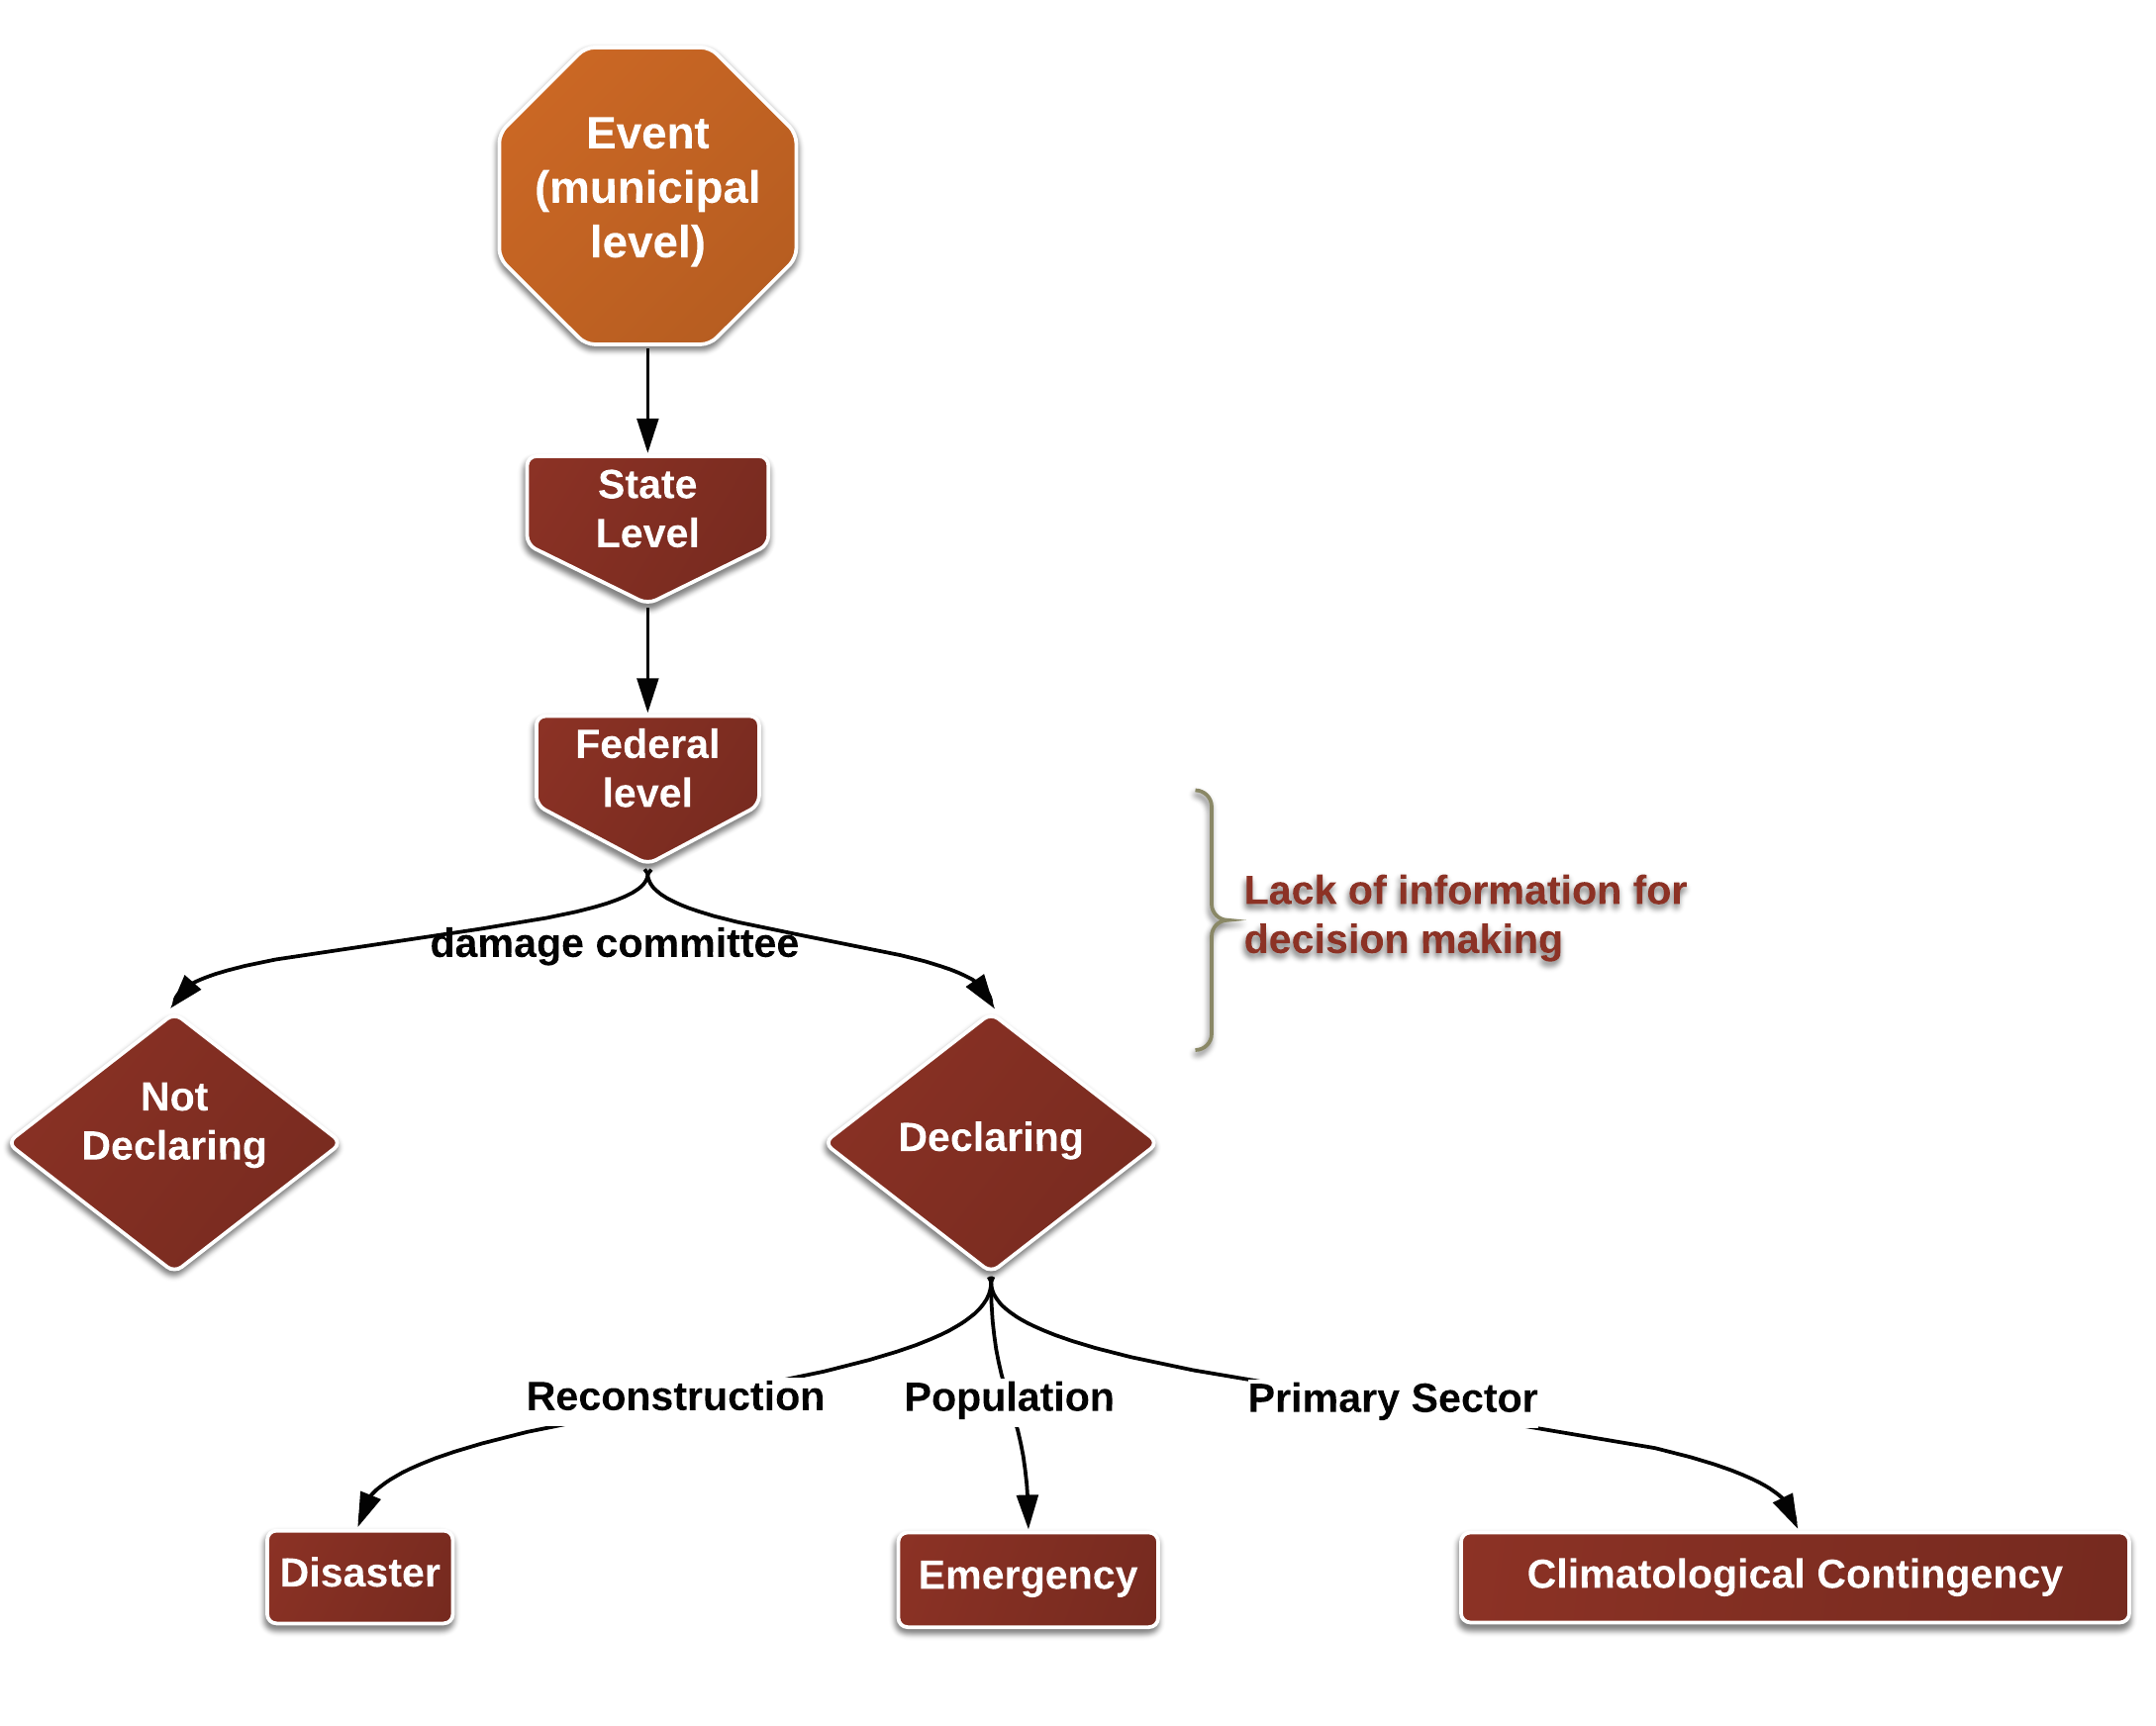
\includegraphics{img/proceso.png}

\end{frame}

\begin{frame}{Problem}

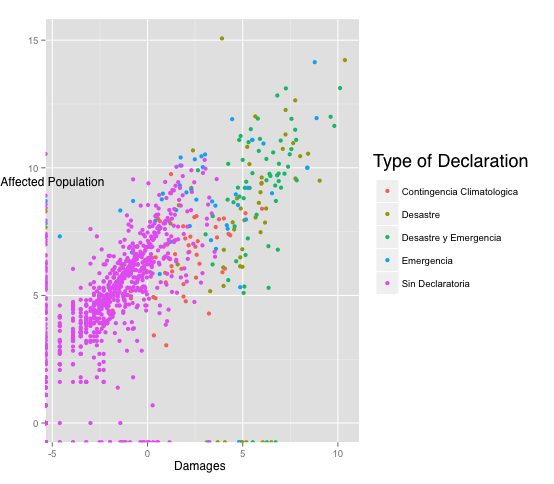
\includegraphics{img/shady.png} 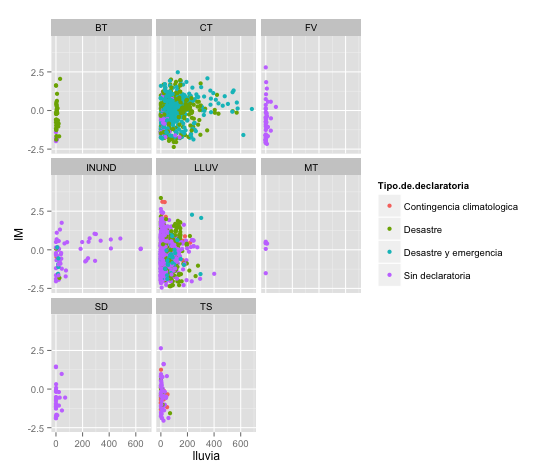
\includegraphics{img/tipo_fen.png}

\end{frame}

\begin{frame}{Objectives}

Develop and apply methods to assess the suitability of using news flows
and precipitation data to characterize disater damages in Mexico looking
forward to resource allocation improvement.

We will work towards an open, real time visualization platform for
coordinated disaster mitigation for decision making.

\end{frame}

\begin{frame}{Working plan}

\begin{itemize}
\itemsep1pt\parskip0pt\parsep0pt
\item
  Analyze information flows using Newspaper, TV and radio data.
\item
  Correlation of news flows with precipitation data.
\item
  Correlation of news flows with damage metrics (evaluation and public
  expenditure).
\item
  Accompanying interactive visualization tools
\end{itemize}

\end{frame}

\begin{frame}{Workflow}

The workflow of the project is the following:

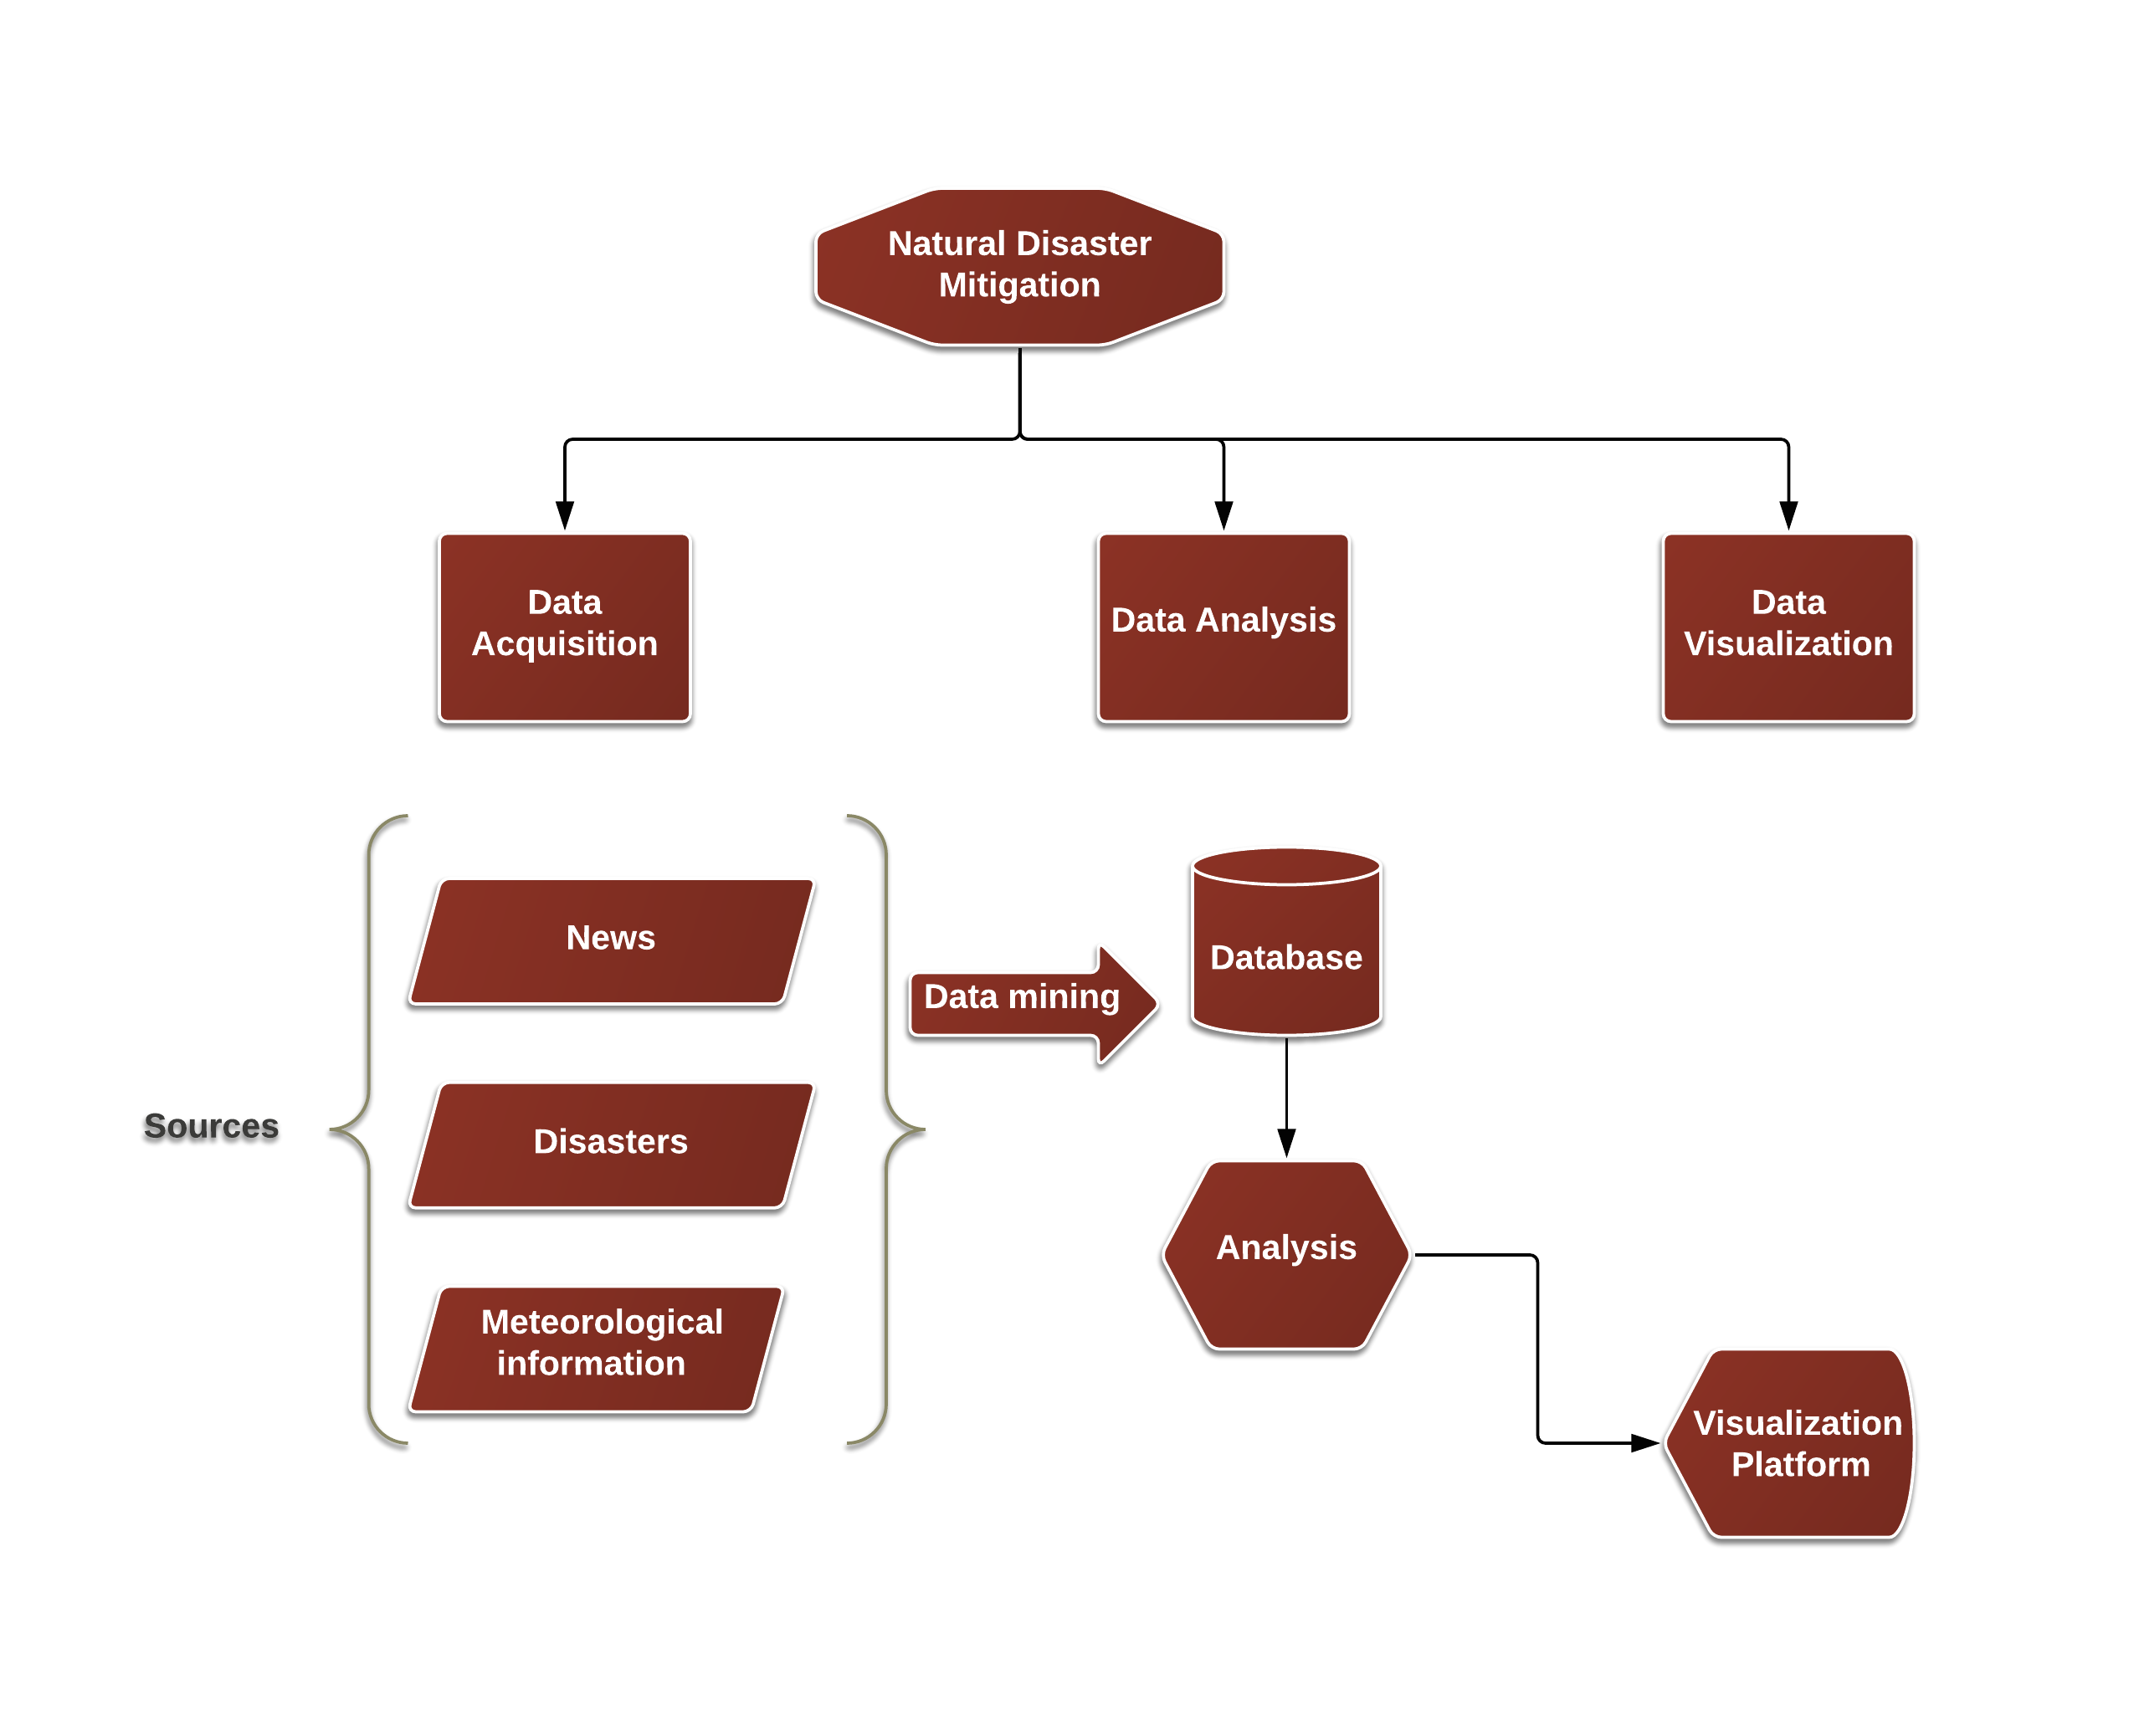
\includegraphics{img/workflow_vf.png}

\end{frame}

\begin{frame}{Information Sources}

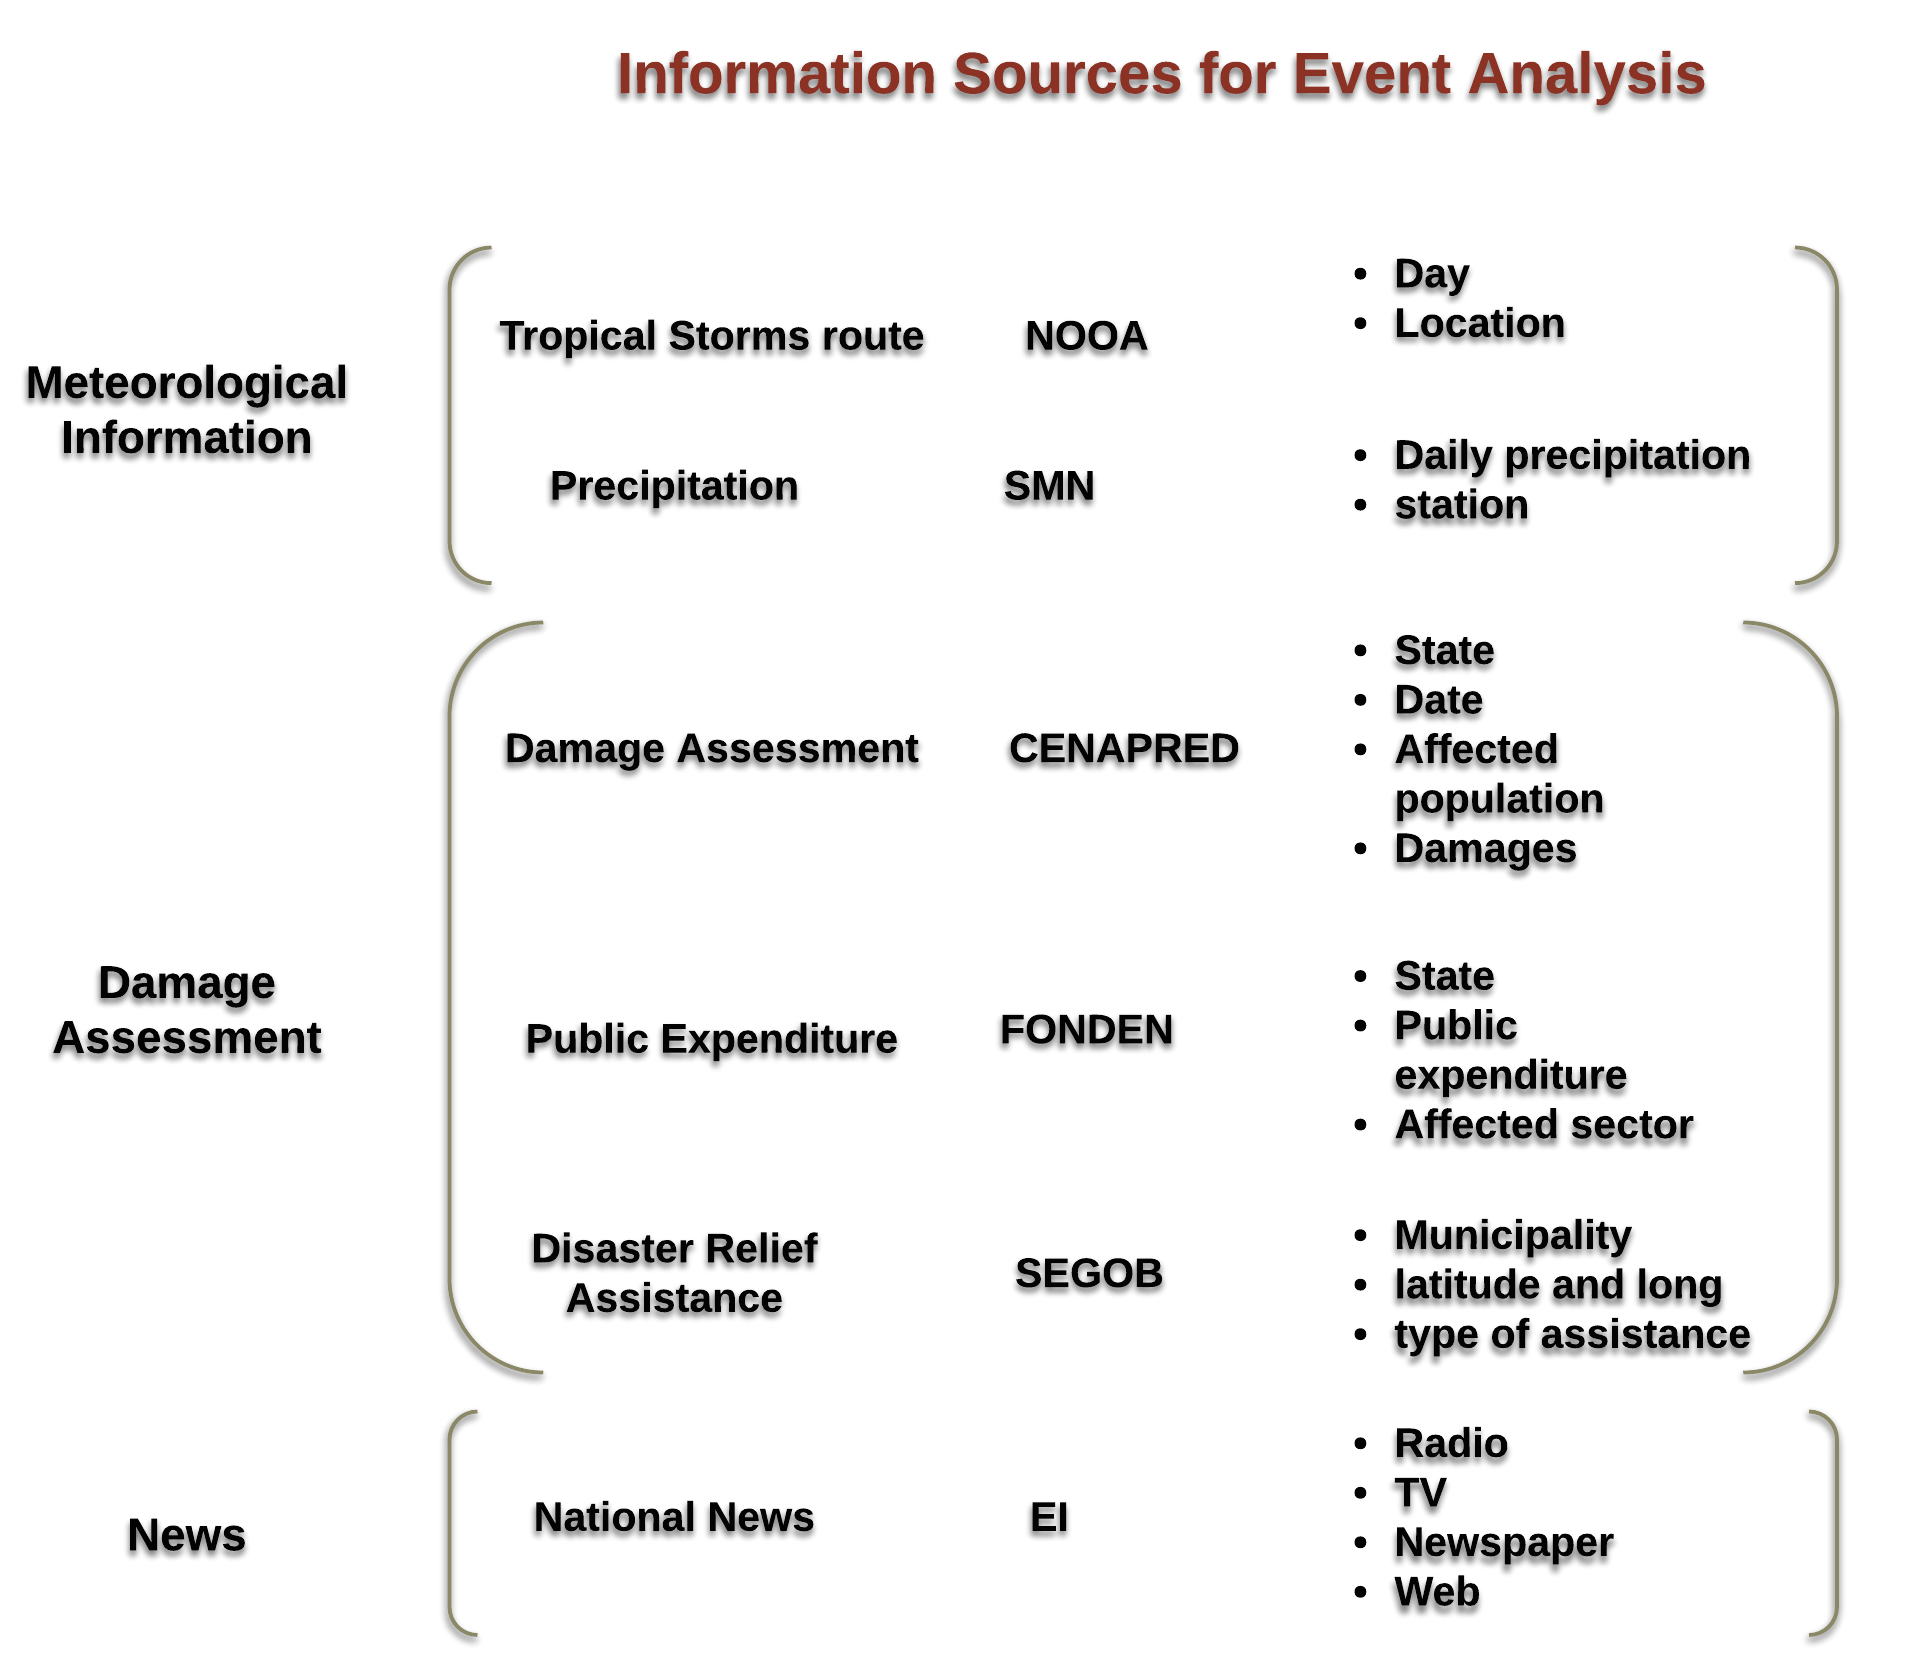
\includegraphics{img/sources.png}

\end{frame}

\begin{frame}{News Porcesing}

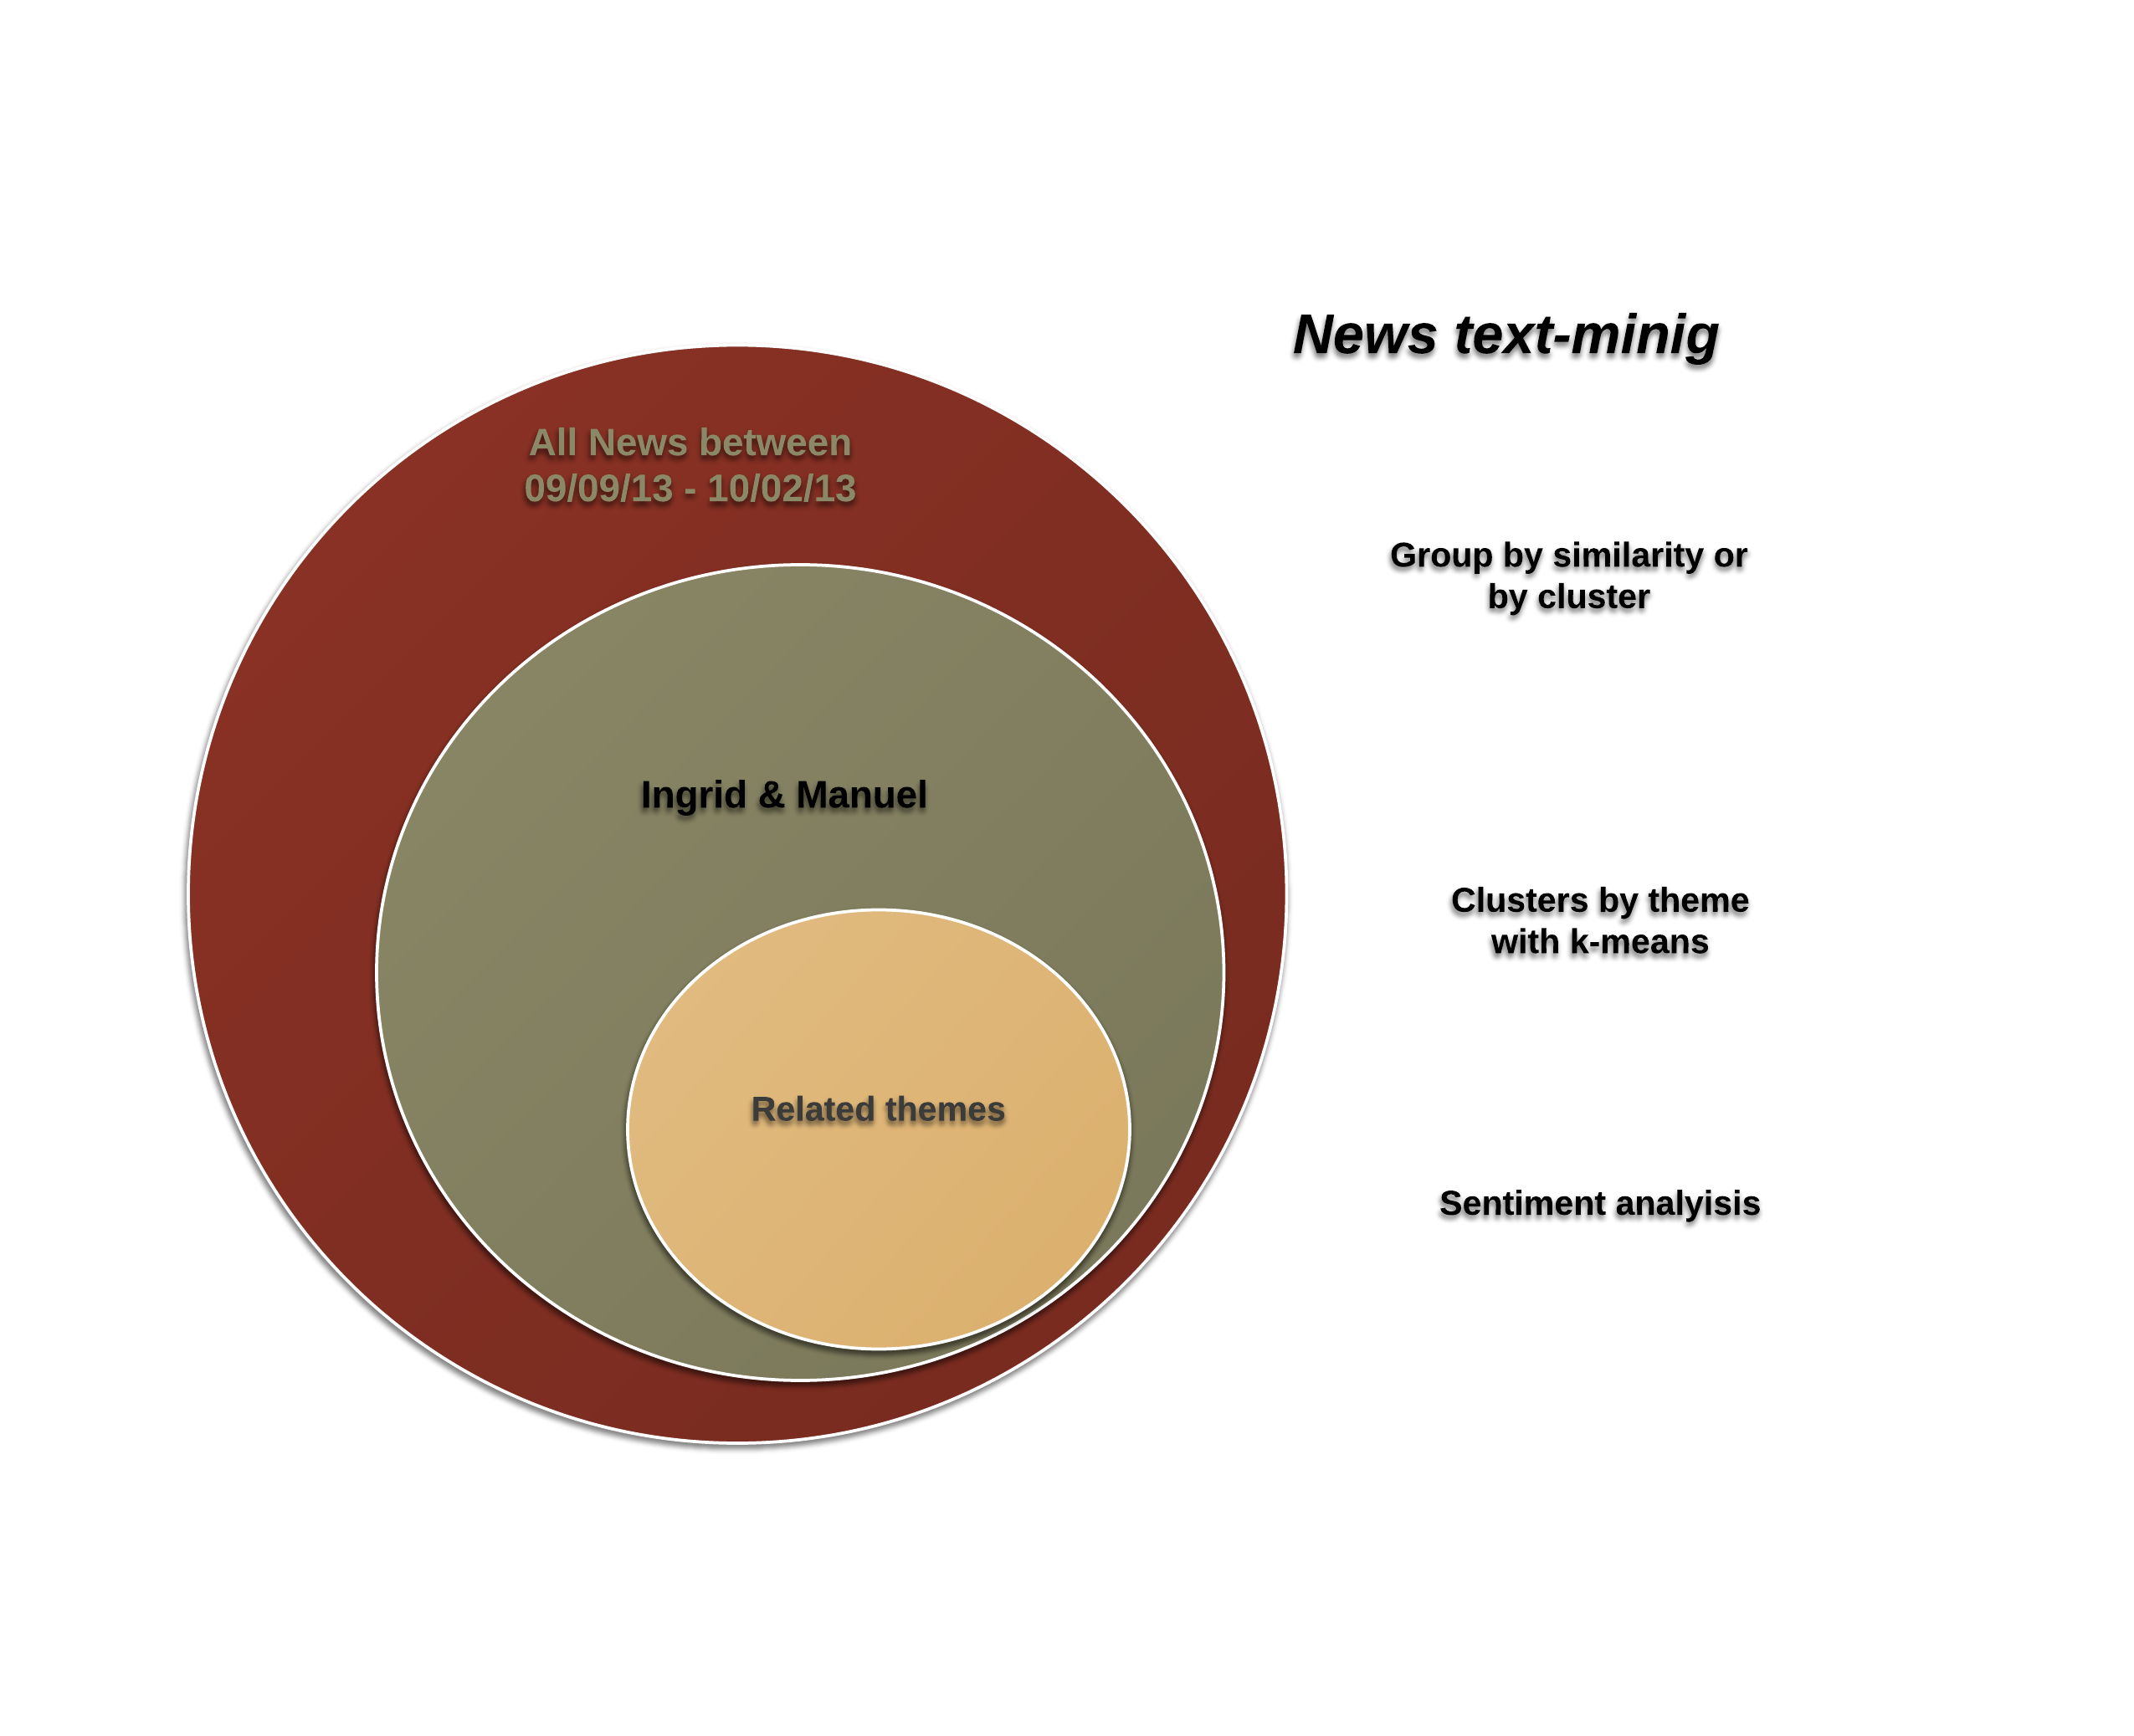
\includegraphics{img/news.png}

\end{frame}

\begin{frame}{Project Time-Line}

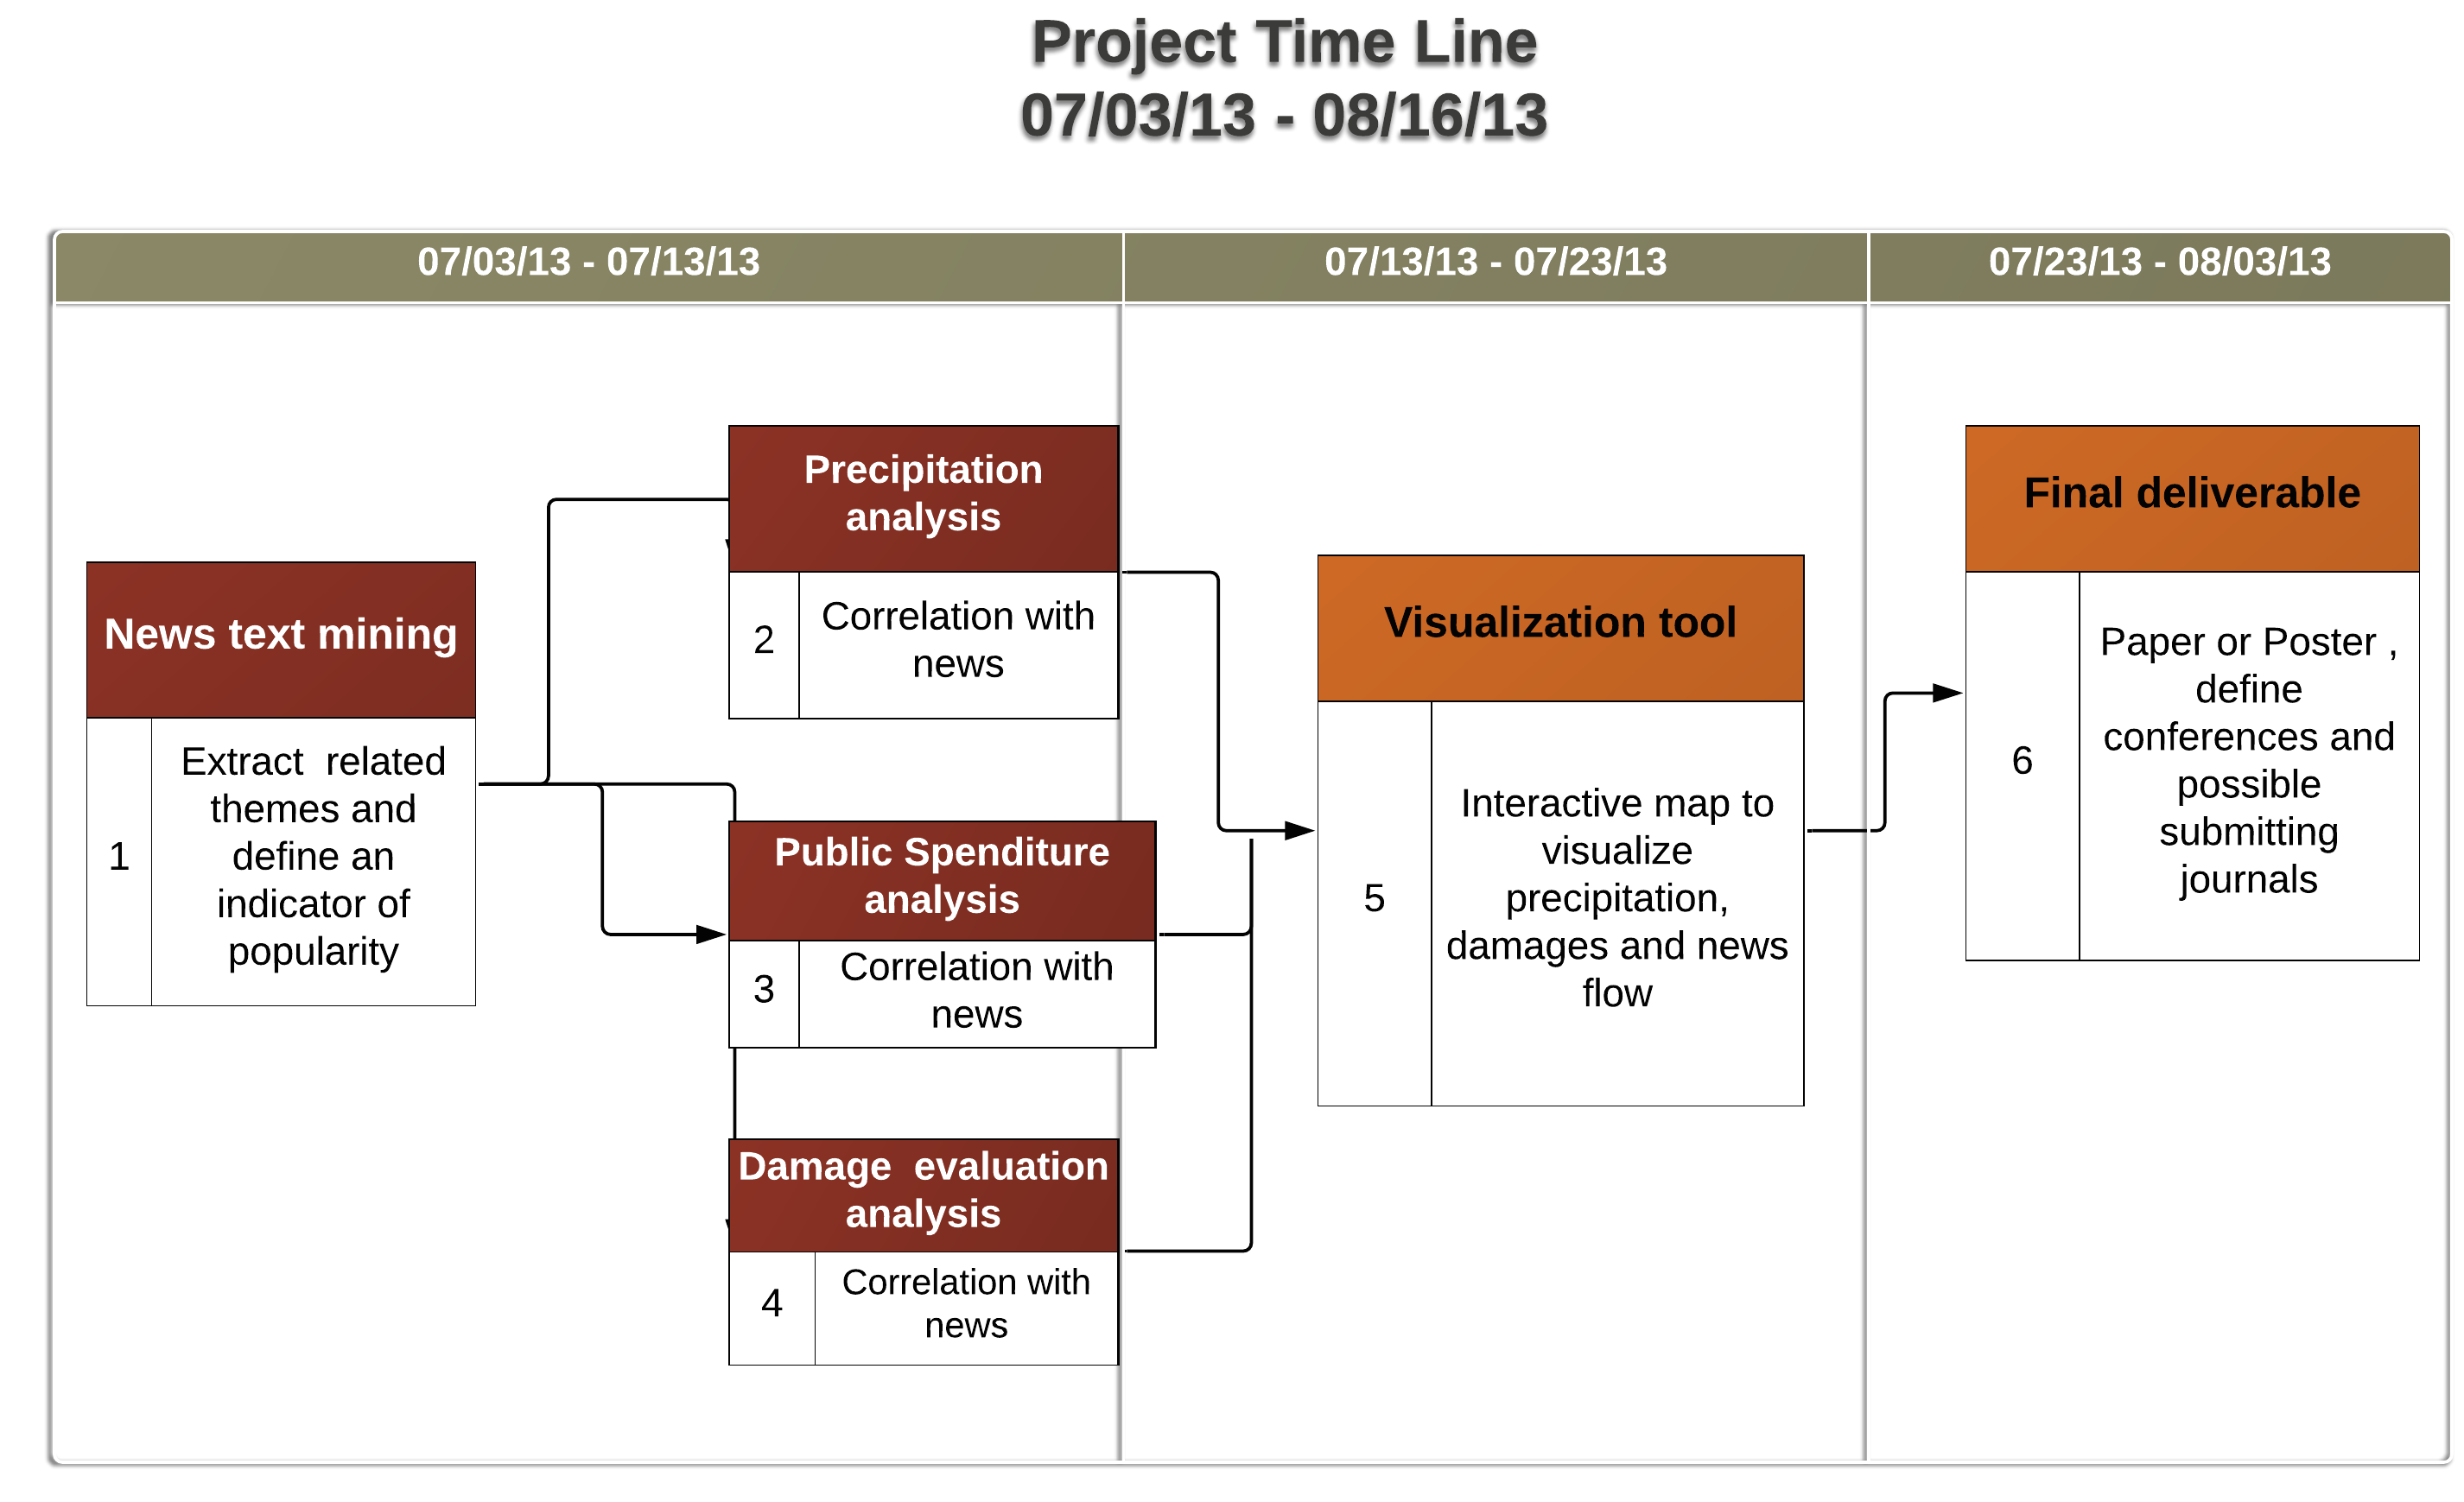
\includegraphics{img/p_tl.png}

\end{frame}

\end{document}
